\documentclass{article}
\usepackage{times}
\usepackage{graphicx}
\usepackage{subfigure} 
\usepackage{natbib}
\usepackage{algorithm}
\usepackage{amsmath}
\usepackage{algorithmic}
\usepackage{subfigure}
\usepackage{hyperref}
\newcommand{\theHalgorithm}{\arabic{algorithm}} % Fixes misbehavior of conflicting packages.
\usepackage{icml2016/icml2016} 
\usepackage[nolist]{acronym} % Acronym package -- give argument <dua> to suppress acronym usage


\icmltitlerunning{Approximate State Abstraction}

% --- Notation Commands ---
\newcommand{\ep}{\widetilde \phi}
\newcommand\defn[1]{{\bf Definition:} #1}


% --- Note Commands ---
\usepackage{color}
\newcommand\dnote[1]{\textcolor{blue}{Dave: #1}}
\newcommand\enote[1]{\textcolor{green}{Ellis: #1}}

% --- DOCUMENT ---
\begin{document}

\twocolumn[
\icmltitle{Approximate State Abstraction}

% Paper Meta Info
\icmlauthor{David Abel}{david_abel@brown.edu}
\icmladdress{Brown University,
            115 Waterman Street, Providence, RI 02906}
\icmlauthor{D. Ellis Hershkowitz}{david_hershkowitz@brown.edu}
\icmladdress{Brown University,
            115 Waterman Street, Providence, RI 02906}
\icmlauthor{Michael L.\ Littman}{michael_littman@brown.edu}
\icmladdress{Brown University,
            115 Waterman Street, Providence, RI 02906}
    
\icmlkeywords{Reinforcement Learning, State Aggregation, State Abstraction, Planning, MDP}
            
\vskip 0.3in
]


%Acronyms -- use \ac for acronym or \acp for plural/capitalization of acronym
\begin{acronym}
\acro{MDP}{Markov Decision Process}
\acrodefplural{MDP}[MDPs]{Markov Decision Processes}

\acro{RL}{reinforcement learning}
\acrodefplural{RL}{RL}{Reinforcement learning}
\end{acronym}


% --- ABSTRACT ---
\begin{abstract}
The combinatorial explosion that plagues planning and \ac{RL} algorithms can be reversed using abstraction. For instance, prohibitively difficult task representations can be condensed so that solutions are tractably computable. In this work, we investigate a theoretical framework for approximate state abstraction that preserves near optimal behavior. \acp{RL} agents using these abstractions may treat experiences that resemble each other as equivalent, and generalize knowledge to novel scenarios based on prior experiences. We present theoretical guarantees of the quality of value functions derived from four classes of approximate state abstraction. Additionally, we empirically evaluate the relationship between the degree of approximation and the degree of abstraction achieved, as well as the tradeoff between approximation magnitude and optimality of behavior.
\end{abstract}

% Set of actions within epsilon (Q*) is the same for two states? Better than boltzmann.


% --- SECTION: Introduction ---
\section{Introduction}
Abstraction is a fundamental tool of intelligent agents seeking to reason about only the salient features of its environment. However, the knowledge available to an agent at any given moment is typically approximate and so agents are faced with the challenge of deciding when their knowledge is sufficiently accurate to form the basis of abstraction. This work focuses on characterizing what ``sufficiently accurate" information for abstraction amounts to in the context of planning and \ac{RL} in \acp{MDP}.

Solving for optimal behavior in \acp{MDP} in a planning setting is known to be P-Complete in the size of the state space~\cite{littman1995complexity,papadimitriou1987complexity}. Similarly, many \ac{RL} algorithms for solving MDPs are known to require a number of samples polynomial in the size of the state space~\cite{strehl2009reinforcement}. Although polynomial runtime or sample complexity is often what one hopes, due to Bellman's so-called curse of dimensionality the state space of an MDP often grows super-polynomially with the number of variables that characterize the domain. Thus, polynomial behavior in state space size is not necessarily the \enote{bee's knees}. For instance, a robot involved in a pick and place task might be able employ planning algorithms to solve for how to manipulate some objects into a desired configuration in time polynomial in the number of states, but the number of states it must consider to do so grows exponentially with the number of objects it plans over CITE DABE ICAPS.

Thus, a key research interest of planning and RL has been leveraging abstraction as means of grappling with large state spaces~\cite{andre2002state,jong2005state,dietterich2000hierarchical,Bean2011}. These methods are characterized by reducing \textit{ground} MDPs with large state spaces to \textit{abstract} MDPs with smaller state spaces by aggregating states with similar values of interest. Existing work has characterized how aggregation of states with equal values of particular quantities fully maintain optimality~\cite{li2006towards,dean1997modelmin}. However, exactly solving for these quantities is itself computationally taxing and sometimes as difficult as solving for optimal behavior in the ground MDP, thereby defeating the purpose of abstraction.

In this work we demonstrate that aggregation of states on the basis of various approximately equal criteria incur bounded error.  Relaxing the aggregation criteria from equality of quantities to epsilon-closeness offers two benefits. First, state aggregation algorithms that satisfy these criteria employ the sort of knowledge which we might reasonably a planning or learning algorithm to approximate without fully solving the MDP. Second, because the state aggregation criteria are relaxed to approximate equality, methods which employ approximate equality are able to tune the aggressiveness of state aggregation all the while incuring bounded error.
	
\enote{ADD QUICK SUMMARY OF PAPER PARAGRAPH}

%\begin{itemize}
%\item Solving MDPs is P-Complete, where the dominant factor is $|\mathcal{S}|$.
%\item Sample complexity is {\it also} dominated by $|\mathcal{S}|$.
%\item To make MDPs with large $|\mathcal{S}|$ tractable, we can reduce the MDPs to a simpler form.
%\item In this work, we show that compressing MDPs in a particular way allows for the transfer of bounded-error solutions between the compressed MDP and ground MDP.
%\item Q: Why approximate?
%\item A: Approximate can compress strictly more than compression based on equality
%\item A: Approximate compression requires the type of knowledge that we could imagine learning (i.e.. approximate knowledge)
%\end{itemize}

% --- SECTION: Background ---
\section{Background}

%MDP/SDM Background and Notation
\subsection{\acp{MDP} and Sequential Decision Making}
A \ac{MDP} is a five-tuple: $\langle \mathcal{S}, \mathcal{A}, \mathcal{T}, \mathcal{R}, \gamma \rangle$: $\mathcal{S}$ is a finite state space; $\mathcal{A}$ is the set of actions available to the agent; $\mathcal{T}$ denotes $\mathcal{T}(s' \mid s,a)$, the probability of an agent applying action $a \in \mathcal{A}$ in state $s \in \mathcal{S}$ and arriving in $s' \in \mathcal{S}$; $\mathcal{R}(s)$ denotes the reward received by the agent arriving in state $s$; $\gamma \in [0, 1]$ is a discount  factor that defines how much the agent prefers immediate rewards over future rewards.

The goal of an agent in an \ac{MDP} is to solve for a policy that maps states to actions: $\pi: \mathcal{S} \rightarrow \mathcal{A}$. In particular, the agent wants to solve for the policy that maximizes its expected discounted reward from any state. This goal policy is denoted $\pi^*$. We denote the expected discounted reward for following policy $\pi$ from state $s$ as the value of the state under that policy, $V(s)^\pi$. We similarly denote the expected discounted reward for taking action $a \in \mathcal{A}$ and then following policy $\pi$ from state $s$ forever after as $Q^\pi(s,a)$. Lastly, we denote the value and $Q$ functions under the optimal policy as $V^*$ and $Q^*$ respectively. \enote{Add citation -- either Littman review paper or Sutton/Barto}

%Lihong Section
\subsection{Abstraction Notation}
We build upon the notation used by \cite{li2006towards} \enote{This should probably say more}.

We understand an abstraction as a mapping from a ground MDP $M_G$ to an abstract MDP $M_A$ using a state aggregation scheme. $M_G = \langle \mathcal{S}_G, \mathcal{A}, \mathcal{T}_G, \mathcal{R}_G, \gamma \rangle$ and $M_A = \langle \mathcal{S}_A, \mathcal{A}, \mathcal{T}_A, \mathcal{R}_A, \gamma \rangle$.

% States
The states in the abstract MDP are constructed by applying a state aggregation scheme, $\phi$, to the states in the ground MDP, $\mathcal{S}_A$. More specifically, $\phi$ maps a state in the ground MDP to a state in the abstract MDP.
\begin{equation}
\mathcal{S}_A = \{ \phi(s) \mid s \in \mathcal{S}_G\}
\end{equation}

Intuitively, the abstract reward function and abstract transition dynamics for each abstract state are a weighted combination of the rewards and transitions for each ground state in the partition. We make now assumptions about the weighting scheme, except that the weighting is a convex combination across all states in partition.

% Reward
The abstract reward function $\mathcal{R}_A(s,a)$ is a weighted sum of the rewards of each of the ground states that map to the abstract state:
\begin{equation}
\mathcal{R}_A(s,a) = \sum_{g \in \phi(s), s \in \mathcal{S}_G} \mathcal{R}_G(g,a) \omega(g) 
\end{equation}


% Transition
The abstract transition function $\mathcal{T}_A(s,a,s')$ is a weighted sum of the transitions of each of the ground states that map to the abstract state:
\begin{equation}
\mathcal{T}_A(s,a,s') = \sum_{g \in \phi^{-1}(s)} \sum_{g' \in \phi^{-1}(s')} \mathcal{T}_G(g,a,g') \omega(g) 
\end{equation}
For:
\begin{equation}
s, s' \in \mathcal{S}_A
\end{equation}

% Abstract policy using in ground.
In general we are interested in how policies defined over the abstract MDP perform in the ground MDP. To leverage a policy defined in the abstract in the ground, we map a ground state into the abstract state space, and query the abstract policy for behavior. Specifically:
\begin{equation}
\pi_A(s) = \pi_A(\phi(s)),\ s \in \mathcal{S}_G
\end{equation}

We evaluate the value of the abstract policy in the ground MDP by following the abstract policy:
\begin{equation}
V^{\pi_A}(s) = \mathcal{R}_G(s,\pi_A(a)) + \gamma \sum_{s' \in \mathcal{S}_G} \mathcal{T}_G(s,\pi_A(a),s')V^{\pi_A}(s')
\end{equation}


\subsection{Exact Abstraction Framework}

\citep{li2006towards} develop a framework for state abstraction in \acp{MDP}, the notation for which is defined in the previous section. Here we survey their main results that we extend to the framework of approximate abstraction.

In particular, they define the following five classes of state abstractors, inspired by existing methods for state abstraction in \acp{MDP}. For brevity, we include those which we build upon directly (see their paper for full details).

\defn{A $Q^*$-irrelevance abstraction, $\phi_{Q^*}$, is such that:
\begin{equation}
\phi_{Q^*}(s_1) = \phi_{Q^*}(s_2) \longrightarrow \forall a\ \left(Q^*(s_1,a) = Q^*(s_2,a)\right)
\end{equation}
}

\defn{A model-irrelevance abstraction, $\phi_{model}$, is such that:
\begin{multline}
\phi_{model}(s_1) = \phi_{model}(s_2) \rightarrow \forall a\ \mathcal{R}_G(s_1,a) = \mathcal{R}_G(s_2,a) \\
\end{multline}
And:
\begin{multline}
\phi_{model}(s_1) = \phi_{model}(s_2) \rightarrow \\ \forall a \sum_{s' \in \phi^{-1}(\phi(s_1))} \mathcal{T}_G(s_1,a,s') =\sum_{s' \in \phi^{-1}(\phi(s_2))} \mathcal{T}_G(s_2,a,s') \\
\end{multline}
}


% --- SECTION: Related Work ---
\section{Related Work}


% Approximate abstraction work.
%Dean: 
%\begin{itemize}
%\item \citep{dean1997model} Does abstraction with model equality.
%\item \citep{dean1997modelmin} Does approximate abstraction with model similarity.
%\end{itemize}
%
%Boutilier:
%\begin{itemize}
%\item ~\citep{dearden1997abstraction} Abstraction: a similar ish bound with a similar is agenda.
%\item ~\citep{Boutilier2000} Stochastic DP: tree based policies, sort of bound thingies.
%\end{itemize}
%
%Even~\cite{even2003approximate}: COLT paper on different metrics
%
%Ortner:
%\begin{itemize}
%\item ~\cite{ortner2013adaptive}: Uses Dean results to do UCRL online learning of abstraction. 
%\item ~\cite{odalric2013optimal}: Learn which abstraction to use online (similar to the Nan paper)
%\end{itemize}


\subsection{Approximate State Abstraction}
\citep{dean1997model} investigates partitioning an MDP's state space into $\epsilon$-homogenous blocks, which are defined as clusters of states whose transition model and reward function are within $\epsilon$ of each other. They provide bounds on the error incurred as a result of using the optimal policy defined over these blocks in the original MDP. This method of abstraction is effectively characterized as a function belonging to the approximate class $\phi_{model}$.
Several approaches build on the notion of $\epsilon$-homogeneity. ~\citep{even2003approximate} analyze different distant metrics used in the process of identifying $\epsilon$-homogenous partitions. ~\cite{ortner2013adaptive} develops an algorithm for learning partitions in an on line setting by taking advantage of the confidence bounds for $T$ and $R$ provided by UCRL~\cite{auer2009near}.

%Prior work considers abstractions related to transition model similarity, or both transition model and reward function similarity with the aim of reducing the state space size required for planning and learning while still achieving a bounded error solution~\cite{even2003approximate,ortner2013adaptive,Boutilier2000}. All of this work is closely in line with our own agenda; they investigate rules for abstractions that may inform a reduced, abstract MDP, the solution to which has bounded error in the original MDP. However, all prior results explore model similarity abstraction rules, whereas we consider several broader classes of approximate abstraction. Furthermore, our results depend on no assumptions regarding the structure of the MDPs in which we apply our abstraction, and generalize to both the reinforcement learning or the planning setting, while many previous approaches require simplifying assumptions about the space of MDPs\dnote{a comment about what assumptions are made would be nice}, or only work target planning.

\subsection{Specific Abstraction Algorithms}
Many previous works have targeted the creation of algorithms that enable state abstraction for MDPs. \citep{andre2002state} investigates a method for state abstraction in hierarchical reinforcement learning leveraging a programming language called ALISP that promotes the notion of {\it safe} state abstraction. Agents programmed using ALISP can ignore irrelevant parts of the state, achieving abstraction that maintains optimality. ~\cite{dietterich2000hierarchical} develops the MAXQ algorithm, a framework for composing tasks into an abstracted hierarchy. \citep{jong2005state} introduce a method called {\it policy-irrelevance}, in which agents identify (online) which state variables may be safely ignored in a factored MDP, and consequently achieve state abstraction. The agent will learn to ignore state variables that don't impact optimal behavior, and is consequently contained within the approximate $\phi_{a^*}$ work. For a full survey of algorithms that leverage state abstraction in recent reinforcement learning literature, see~\cite{li2006towards}.


% Other? Selecting abstractions
%\subsection{Selecting Abstractions}
%\citep{jiang2015abstraction} investigate the question of choosing between two abstractions during learning. They provide analysis for an online approach to identifying the better abstraction. 

% Defining 

% Critically, our work differs from these in that our primary aim is to achieve understanding of what methods of abstraction in reinforcement learning can maintain bounded error solutions, while these focus on particular strategies that fit within our framework.

% Lihong/Walsh/Littman: Towards a unified theory...

%\begin{itemize}
%\item {\bf Approximate equivalence of MDP}~\cite{even2003approximate}
%\item ALisp~\cite{andre2002state}
%\item Aggregation in DP~\cite{Bean2011}
%\item {\bf Does approximate aggregation and then UCRL}~\cite{ortner2013adaptive}
%Very similar to our overall goal: learn an abstraction function online using confidence bounds as the epsilon. Wowza. Only uses the whole model similarity business though. Seems to be the case for all of the approximate aggregation work (just does the bisimulation or $\epsilon-homogeneity$)
%
%\item Selecting the state rep in RL~\cite{maillard2011selecting}
%\item Near optimal state reps~\cite{ortner2014selecting}
%\item SMDP homomorphisms~\cite{ravindran2003smdp}
%\end{itemize}


% --- SECTION: State Abstraction ---
\section{Approximate State Abstraction}

% Explain each of the Phis

% One theorem, each separate phi is its own lemma.

% Proof of Q^*

% Possibly a lemma for NP-Completeness of the minimal such phi for all abstractions (was a result for model in previous cases).

% Subsections for proofs for each phi
\dnote{Insert lemma for each phi as their subsection, maybe with proof sketch but likely just dump in appendix.}

% Subsection: 

% Subsection: Phi_Q
\subsection{$\phi_{Q^*}$}

% Subsection: Phi_M
\subsection{$\phi_{model}$}

% Subsection: Phi_{Mult}
\subsection{$\phi_{mult}$}

% Subsection: Phi_B
\subsection{$\phi_{bolt}$}

% Subsection: Other Abstractions
\subsection{Other Abstractions}

We note that one natural way of approximating $\phi_{a^*}$ from ~\cite{li2006towards}, in which states that are compressed together share optimal actions and the Q values of these actions are within $\varepsilon$ is ultimately equivalent to the crisp abstraction $\phi_{\pi^*}$, in states that are compressed share an optimal action. A true approximation of $\phi_{a^*}$ ought to also approximate the optimality of each action. Given the degree of compression achievable under $\phi_{a^*}$, especially with temporally extended actions, we foresee this approximate form of abstraction as being of great interest, and plan to investigate it in future work.

We are {\it not} going to provide results for $\phi_{\pi^*}$, since relaxing equality of optimal actions doesn't mean anything.

Additionally, we are {\it not} going to provide results for $\phi_{Q^\pi}$, since as Lihong's paper notes, ``It is an open question how to find $Q^\pi$ irrelevance abstractions without enumerating all possible policies, they do not give results. Furthermore, an MDP for which this is true is an awfully weird MDP...

Lastly, we are interested in a generalization of $\phi_{mult}$  and $\phi_{bolt}$ that handles a broader space of distributions over Q values.


% Some abstractions DON'T preserve a meaningful notion of optimality.



% --- SECTION: Example Domains ---
\section{Example Domains}

\dnote{For each section, we'll include a plot comparing $\epsilon$ to \# states, and $\epsilon$ to performance. For UpWorld and NChain, we can include visuals of uncompressed and compressed (not useful for trench).}

% Subsection: UpWorld
\subsection{UpWorld}

\dnote{As part of UpWorld we can include the result about the unbounded improvement in sample complexity (small lemma or something?)}

% Insert visual and/or stats on number of states and performance of VI solving the abstract MDP and evaluating the resulting policy on the original MDP


% Subsection: NChain
\subsection{NChain}

% Insert visual and/or stats on number of states and performance of VI solving the abstract MDP and evaluating the resulting policy on the original MDP


% Subsection: Trench
\subsection{Trench}

% Insert visual and/or stats on number of states and performance of VI solving the abstract MDP and evaluating the resulting policy on the original MDP


% Figure: The Trench Problem
\begin{figure}[h]
\centering
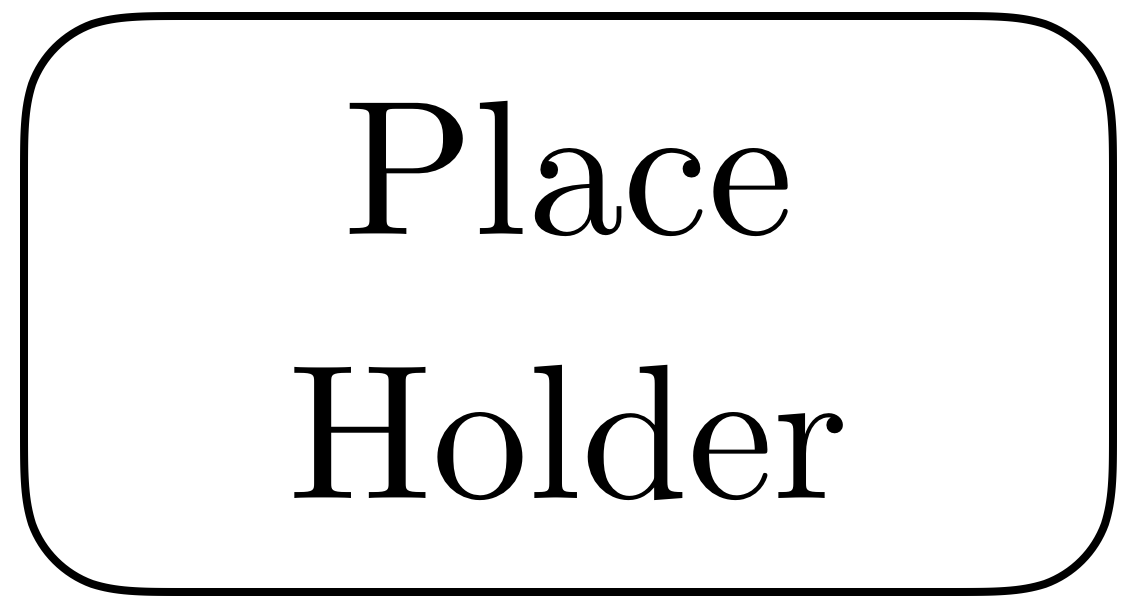
\includegraphics[width=0.42\columnwidth]{figures/placeholder.png}
\caption{The Trench Problem}
\label{fig:trench}
\end{figure}


% --- SECTION: Approximate Abstraction on Example Domains ---
\section{Approximate Abstraction on Example Domains}

% Figure: Epsilon vs. #States for all three sample domains.
\begin{figure}
\subfigure[UpWorld]{
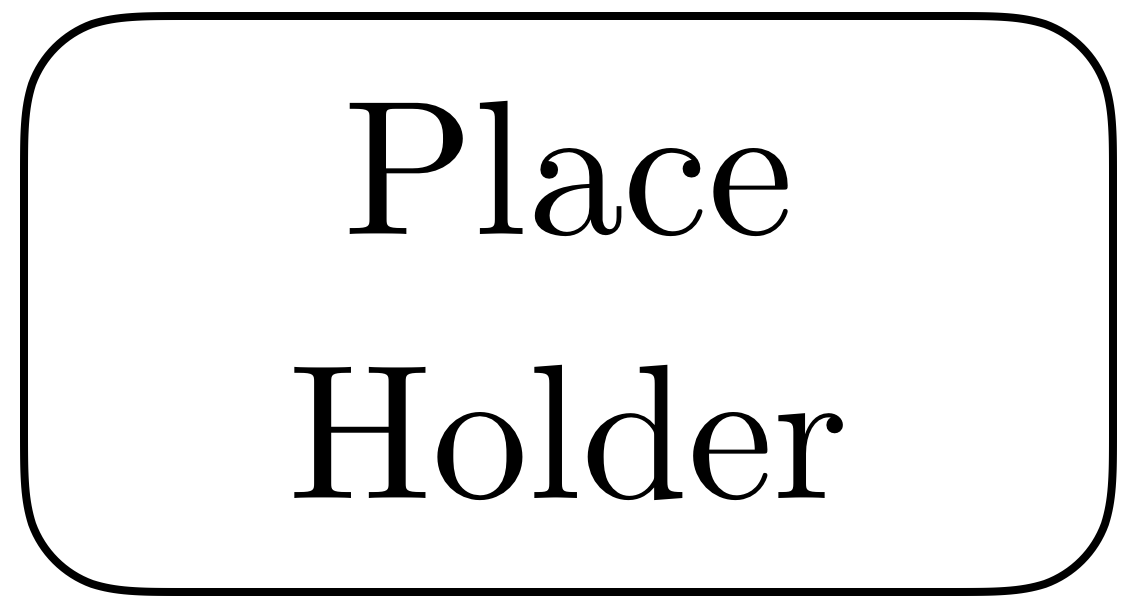
\includegraphics[width=0.28\columnwidth]{figures/placeholder.png}}
\subfigure[NChain]{
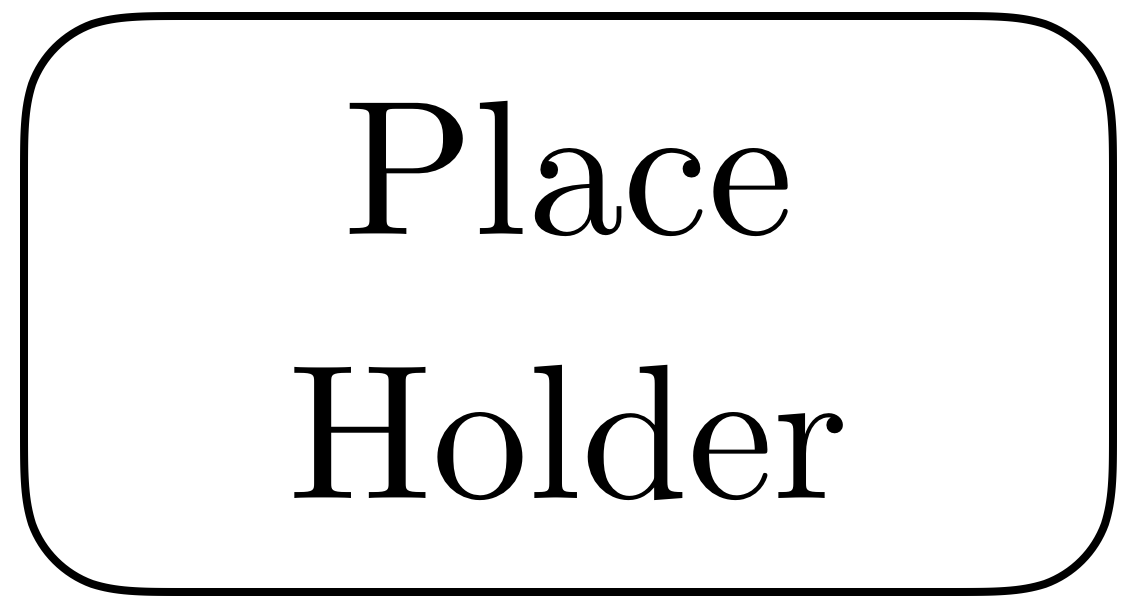
\includegraphics[width=0.28\columnwidth]{figures/placeholder.png}}
\subfigure[Trench]{
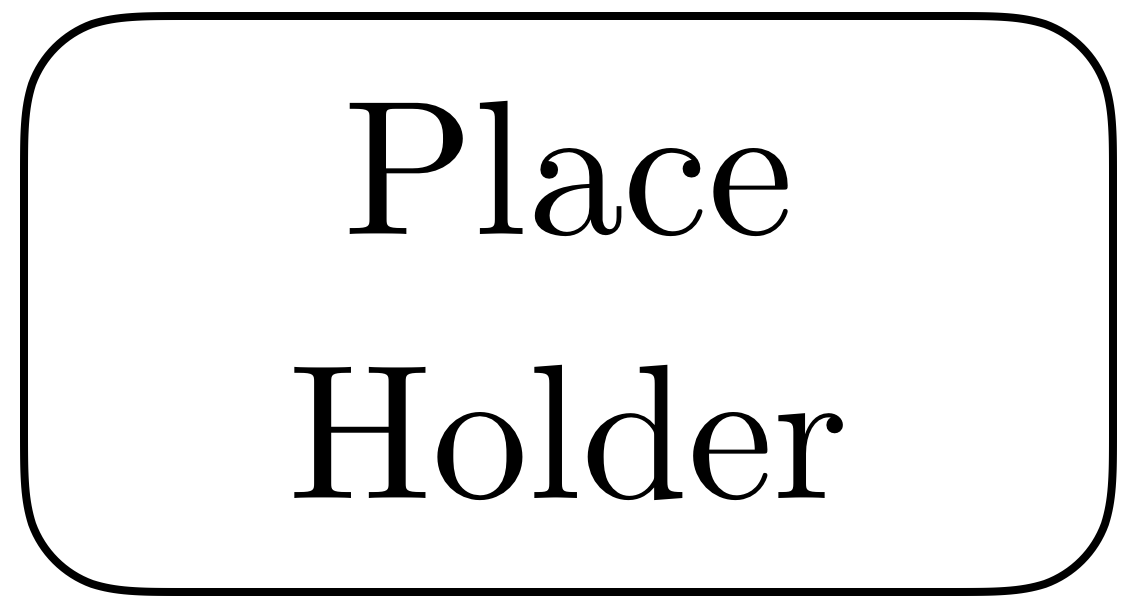
\includegraphics[width=0.28\columnwidth]{figures/placeholder.png}}
\label{fig:eps-states}
\caption{$\epsilon$ vs. Num States}
\end{figure} 

% Figure: Epsilon vs. Error in Abstract Value Function
\begin{figure}
\subfigure[UpWorld]{
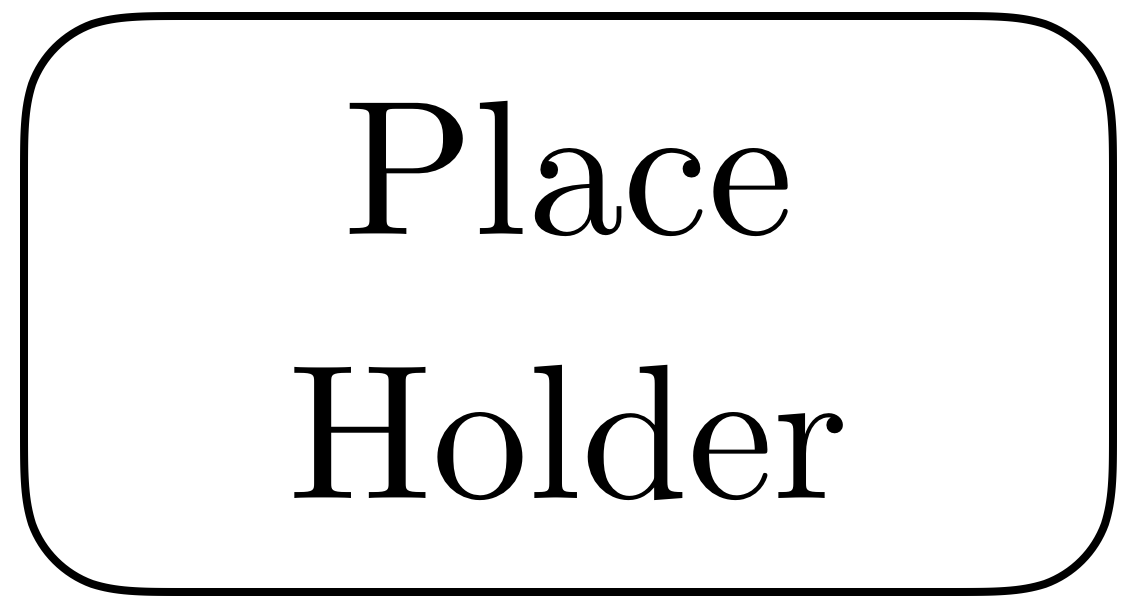
\includegraphics[width=0.28\columnwidth]{figures/placeholder.png}}
\subfigure[NChain]{
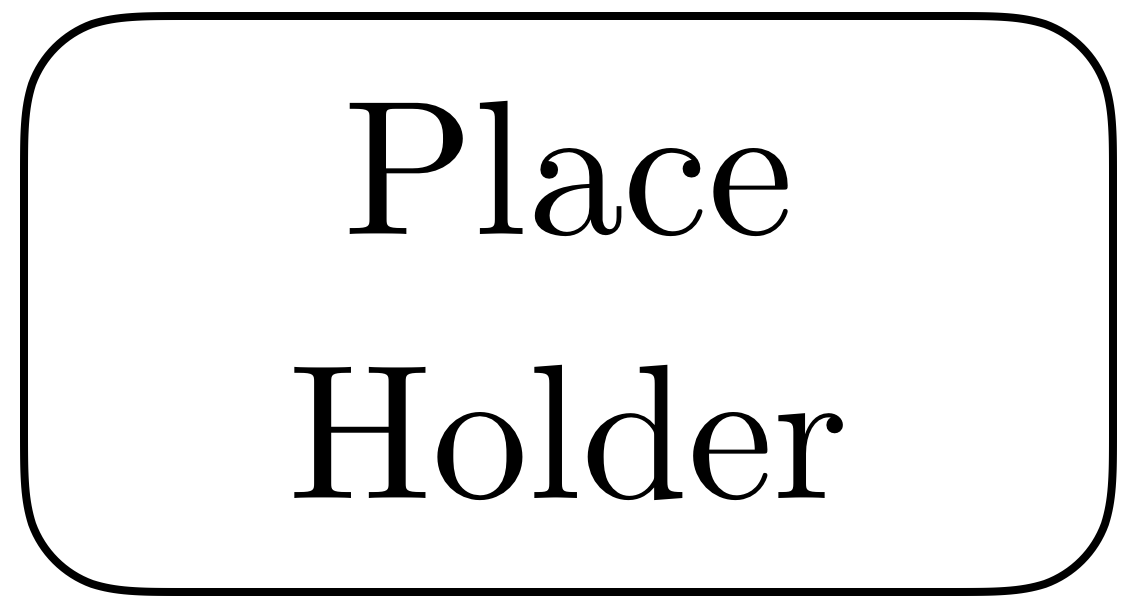
\includegraphics[width=0.28\columnwidth]{figures/placeholder.png}}
\subfigure[Trench]{
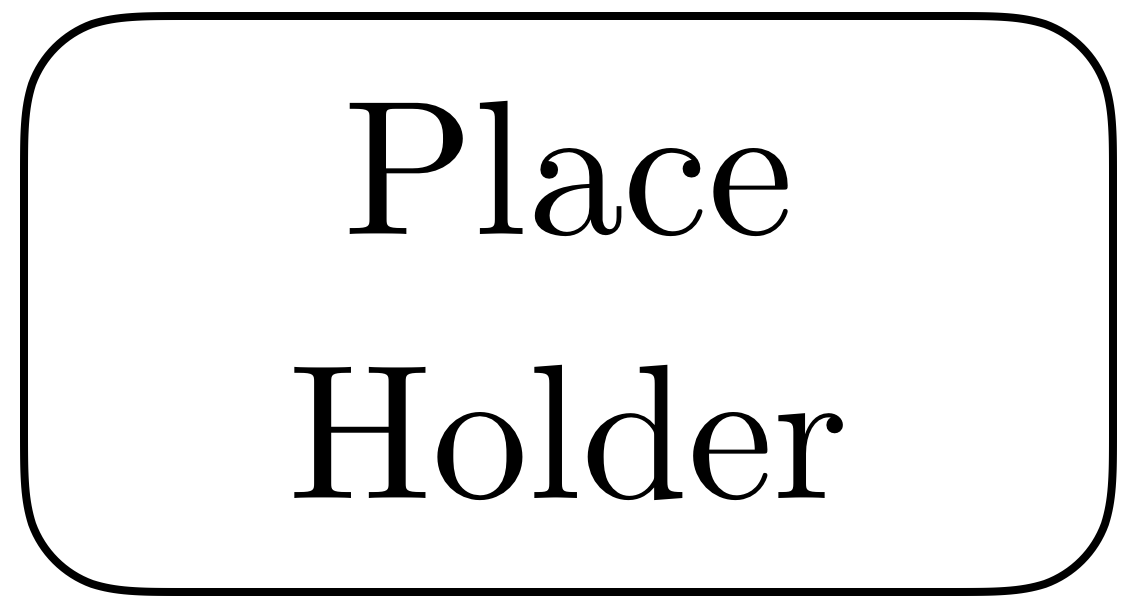
\includegraphics[width=0.28\columnwidth]{figures/placeholder.png}}
\label{fig:eps-states}
\caption{$\epsilon$ vs. Error in Abstract Value Function}
\end{figure} 



% Subsection: Abstract Domain Visualizations
\subsection{Abstract Domain Visualizations}

% Figure: UpWorld MDP visuals
\begin{figure}[h]
\centering
\subfigure[UpWorld]{
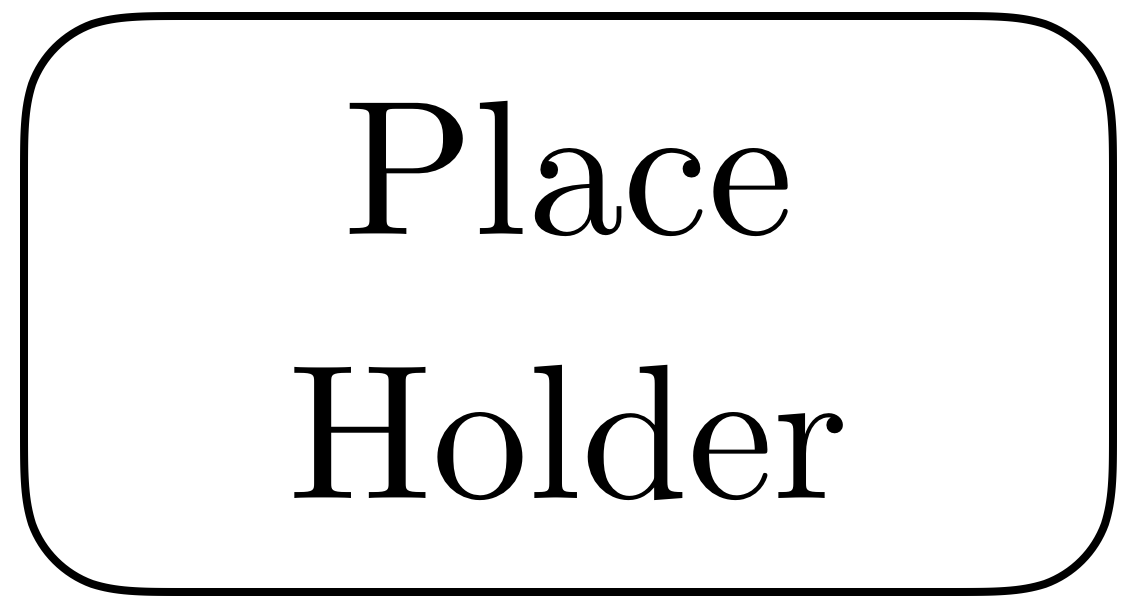
\includegraphics[width=0.46\columnwidth]{figures/placeholder.png}}
\hspace{3mm}
\subfigure[Abstracted UpWorld]{
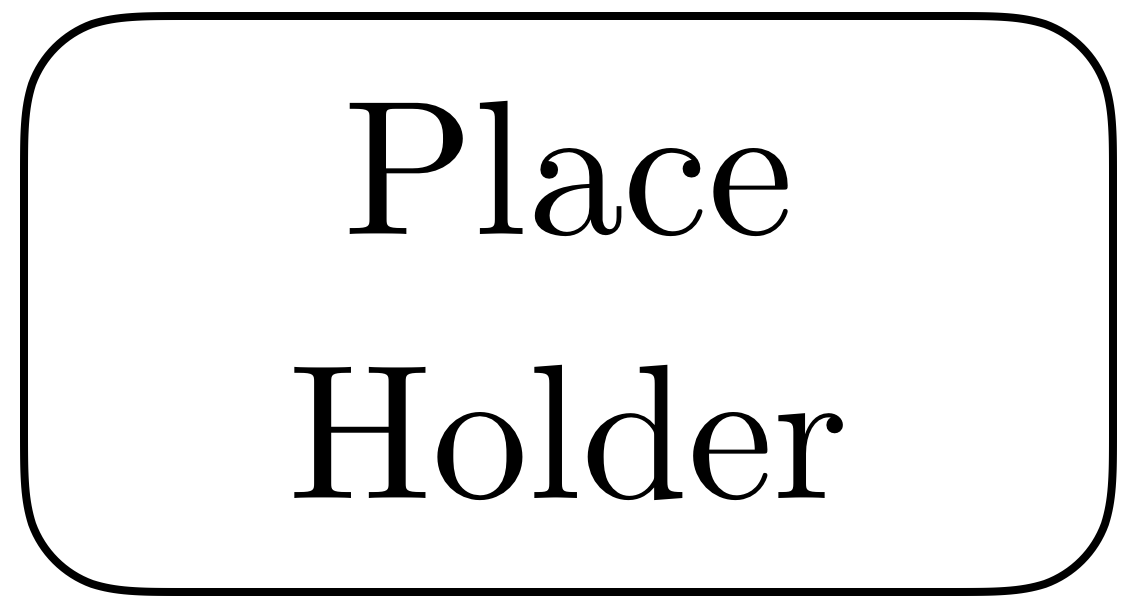
\includegraphics[width=0.46\columnwidth]{figures/placeholder.png}}
\caption{Visualization of Original UpWorld vs. Abstracted UpWorld}
\end{figure}

% Figure: NChain MDP visuals
\begin{figure}[h]
\centering
\subfigure[NChain]{
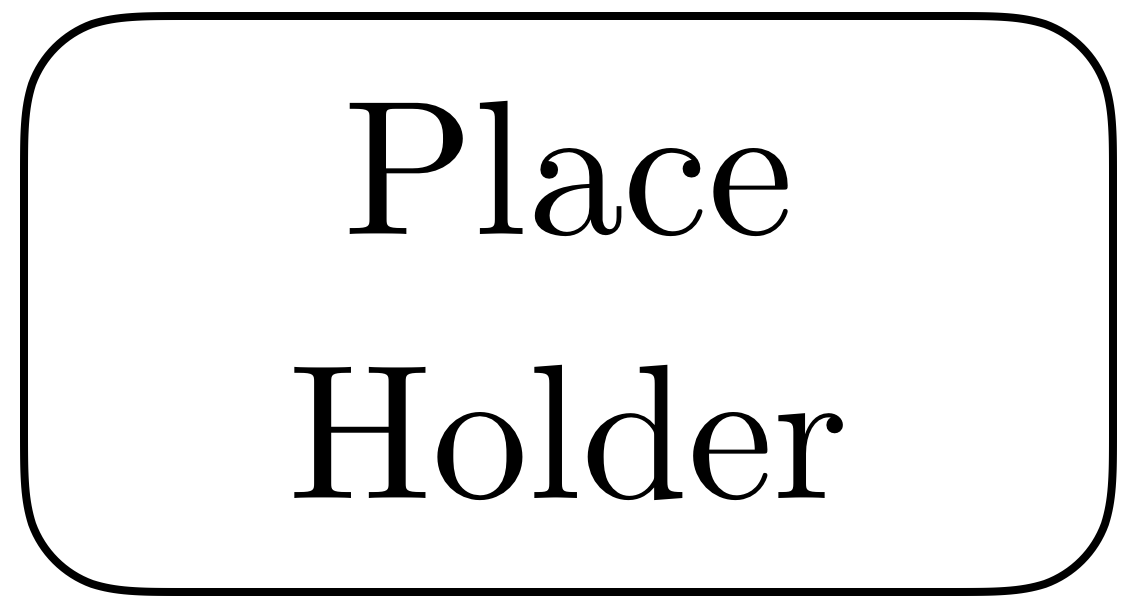
\includegraphics[width=0.46\columnwidth]{figures/placeholder.png}}
\hspace{3mm}
\subfigure[Abstracted NChain ]{
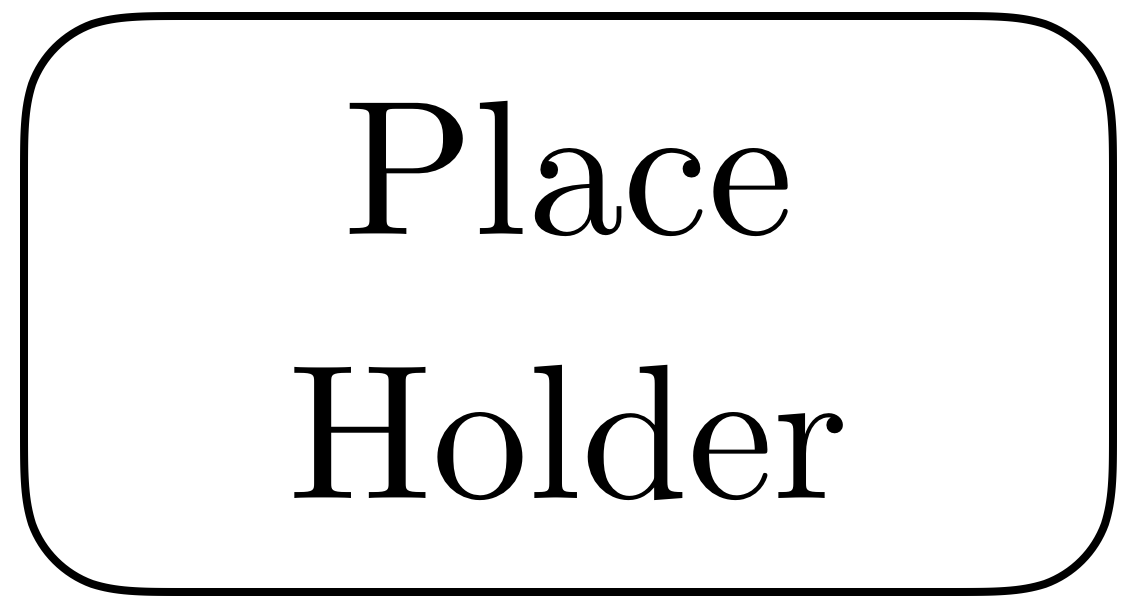
\includegraphics[width=0.46\columnwidth]{figures/placeholder.png}}
\caption{Visualization of Original NChain vs. Abstracted NChain}
\end{figure}






% --- SECTION: Conclusion ---
\section{Conclusion}

% Summary

% Future Work
\begin{enumerate}
\item Learning Phi
\begin{itemize}
\item Exploration vs. Exploitation problem is different while trying to learn Phi
\end{itemize}
\item Compressibility
\begin{itemize}
\item Relationship between approximate abstract and compressibility
\end{itemize}
\item POMDP and abstraction
\end{enumerate}





% --- BIBLIOGRAPHY ---
\bibliographystyle{icml2016/icml2016}
\bibliography{state_abs}

\end{document}
